
\section{Theory}

\subsection{Single Particle Dynamics}

When working with beams of particles, it is advantageous to work in the
coordinate system that follows the ideal path of the beam, denoting that axis by
\(z\). If the beam's motion in the transverse \(x\) and \(y\) planes are
independent, i.e. we ignore coupling terms, the each particle's motion in each
plane can be described by
\begin{equation}
	\begin{pmatrix}
		u(z) \\ u'(z)
	\end{pmatrix}
	=
	\begin{pmatrix}
		C_u(z)  & S_u(z)  \\
		C'_u(z) & S'_u(z)
	\end{pmatrix}
	\begin{pmatrix}
		u_0 \\ u'_0
	\end{pmatrix}
\end{equation}
where \(u\) is either \(x\) or \(y\) and \(u'\) is the transverse velocity of
the particle in the \(u\) plane. The coordinate \((u, u')\) lies in what is
known as phase space. Using this system of matricies the drift and quadrupole
matricies can be derived \cite{wiedemann2007particle}. The drift matrix is
\begin{equation}
	\mathcal{M}_D(l) =
	\begin{pmatrix}
		1 & l \\
		0 & 1
	\end{pmatrix}
	\label{eq:drift}
\end{equation}
the focusing quadrupole matrix is
\begin{equation}
	\mathcal{M}_{QF}(l) =
	\begin{pmatrix}
		\cos\psi & \frac{1}{\sqrt{k}}\sin\psi \\
		-\sqrt{k}\sin\psi & \cos\psi
	\end{pmatrix}
	\label{eq:qf}
\end{equation}
and the defocusing quadrupole matrix is
\begin{equation}
	\mathcal{M}_{QD}(l) =
	\begin{pmatrix}
		\cosh\psi & \frac{1}{\sqrt{\abs{k}}}\sinh\psi \\
		-\sqrt{\abs{k}}\sinh\psi & \cosh\psi
	\end{pmatrix}
	\label{eq:qd}
\end{equation}

These transport matricies can be multiplied together resulting in the
transformation matrix representing all the components of a beamline making it
simple to follow a particle through a transport line.
% TODO confusing sentence

\subsection{Emittance}
\label{sec:emittance}

\begin{figure}
	\centering
	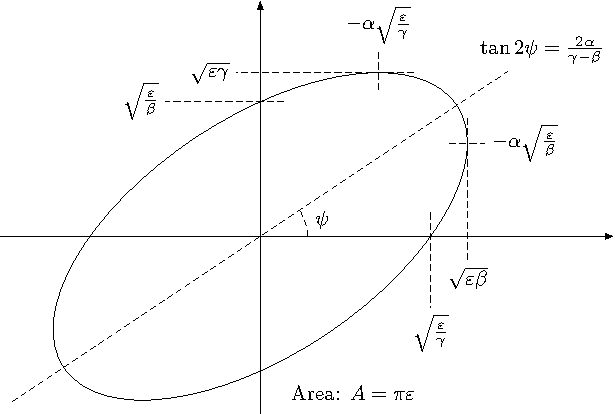
\includegraphics{figures/ellipse}
	\caption{
		A representation of the relation between the Twiss parameters of
		a beam's ellipse in phase space~\cite{wiedemann2007particle}.}
	\label{fig:ellipse}
\end{figure}

Grouping the individual particles in a particle beam, they will occupy an area
in phase space known as the emittance.  Qualitatively the emittance of a beam is
a measure of how parallel the particles of the beam are to each other and is a
conserved quantity while the beam is not being acted upon by external forces.

In phase space the beam of particles will usually take up an area resembling
that of an ellipse. This is because, after a diverging or converging beam has
traveled through an aperture, we expect particles that are further away from the
centre of the beam to have a larger transverse momentum. This is unless the beam
is being measured at it's waist where it is transitioning between converging and
diverging or visa versa. Figure~\ref{fig:ellipse} shows the projection of a
diverging beam onto a two dimensional phase plane, called the phase ellipse.
The line that defines the ellipse is drawn such that \SI{95}{\percent} of all
the particles in the beam are contained within it~\cite{buon1994beam}. The
emittance is defined by the area of this ellipse divided by \(\pi\) in units of
\si{\meter\radian}. Note that in general, the transverse momenta, hence the
slope of the particles in the beam, are very small so the approximation \(\sin
u'\approx u'\) can be used.
% TODO explain angle or transverse momentum on y axis in phase space

% \begin{equation}
% 	\int_{\text{ellipse}}\mathrm{d}x\mathrm{d}x' =\pi\epsilon
% \end{equation}

The general equation of an ellipse can be used to describe the phase ellipse:
\begin{equation}
	\gamma x^2 + 2\alpha xx' + \beta x'^2 = \epsilon
\end{equation}
where \(\alpha\),  \(\beta\), \(\gamma\) and \(\epsilon\) are ellipse parameters
that determine the ellipse's shape and orientation in phase space, where
\(\epsilon\), the area of the ellipse is the emittance~\footnote{Often, the
units of \(\pi\) are omitted and the emittance is given in units of
\si{\pi\;\meter\;\radian}.}. Of the four beam parameters, only three are
independent and since \(\epsilon\) is defined as the area, the other three can
be found to be correlated from the ellipse's geometric properties by
\begin{equation}
	\beta\gamma - \alpha^2 = 1
\end{equation}

% \subsection{Methods of measurement}

% The phase-space density and emittance of a beam must be infered from beam
% profiles captured using charge-coupled device (CCD) cameras after undergoing
% spatial filtering.

% By expressing this ellipse as a matrix,
A matrix describing the beam has been derived from the matirix representation of
the ellipse to transport the beam via the transport matricies in
Equations~(\ref{eq:drift}), (\ref{eq:qd}) and
(\ref{eq:qf})~\cite{wiedemann2007particle}. This beam matrix is defined by
\begin{equation}
	\bm{\sigma} =
	\begin{pmatrix}
		\sigma_{11} & \sigma_{12} \\
		\sigma_{21} & \sigma_{22} \\
	\end{pmatrix}
	=
	\epsilon
	\begin{pmatrix}
		\beta & -\alpha \\
		-\alpha & \gamma \\
	\end{pmatrix}
\end{equation}
where each element describes distributions of particles in the beam as follows:
\begin{align}
	\sigma_{11} &= \langle x_i^2 \rangle = \epsilon\beta \\
	\sigma_{22} &= \langle {x'}_i^2 \rangle = \epsilon\gamma \\
	\sigma_{12} &= \langle x_i x'_i \rangle = -\epsilon\alpha
\end{align}

The evolution of this matrix along the beam transport line can then be described
by
\begin{equation}
	\bm{\sigma}_1 = \mathcal{M}\;\bm{\sigma}_0\;\mathcal{M}^T
	\label{eq:apply}
\end{equation}
where \(\bm{\sigma}_0\) is the initial beam matrix, \(\mathcal{M}\) is the
transport matrix of the beam line and \(\bm{\sigma}_1\) is the beam matrix at
the end of the beam line.

% TODO measurement of the emittance 183gg (page 164)
